\section{Student Survey}

\paragraph{}
\noindent\textbf{WPI George C. Gordon Library Mobile App}
\newline
\noindent Our IQP team is investigating the development of a mobile library app. We are seeking your feedback on the potential resources and services WPI users would utilize in this app.
All responses to the survey are completely anonymous, and cannot be traced back to the respondent. You may however, provide your WPI email address at the end, and we may contact you to discuss additional ideas. 
If you have any questions or concerns about this survey or project, please choose to contact us at:
gr-libappteam@wpi.edu
*All of the following questions and the entire survey are both completely optional*
\newline


\noindent\textbf{Question 1: What is your current academic status at WPI?}
\begin{itemize}
    \item Certificate
    \item Undergraduate
    \item Master's
    \item PhD
    \item Other:
\end{itemize}
\newline


\noindent\textbf{Question 2: What is your declared major?}
\paragraph{}
Choose
\newline


\noindent\textbf{Question 3: What is your current enrollment status?}
\begin{itemize}
    \item Full-time
    \item Part-time
    \item Not currently enrolled
\end{itemize}
\newline


\noindent\textbf{Question 4: How often do you currently use the following services or information?}
\begin{figure}[H]
    \centering
     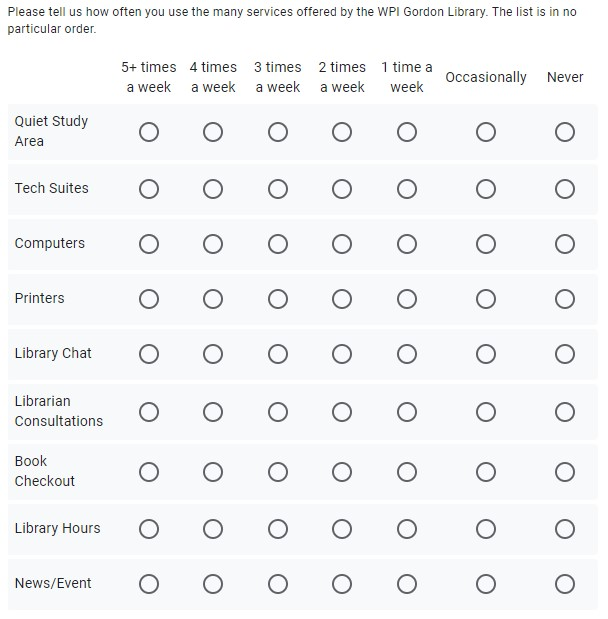
\includegraphics[width = \textwidth, height = \textheight, keepaspectratio]{assets/img/Initial Survey Q4.jpg}
\end{figure}
\newline


\noindent\textbf{Question 5: Would you use a mobile app for the WPI Gordon Library?}
\begin{itemize}
    \item Yes
    \item No
    \item Maybe
\end{itemize}
\newline


\noindent\textbf{Question 6: If answered "no" to the previous question, please explain why.}
\paragraph{}
Your answer
\newline


\noindent\textbf{Question 7: What are some features you would utilize in a library mobile app?}
\begin{figure}[H]
    \centering
     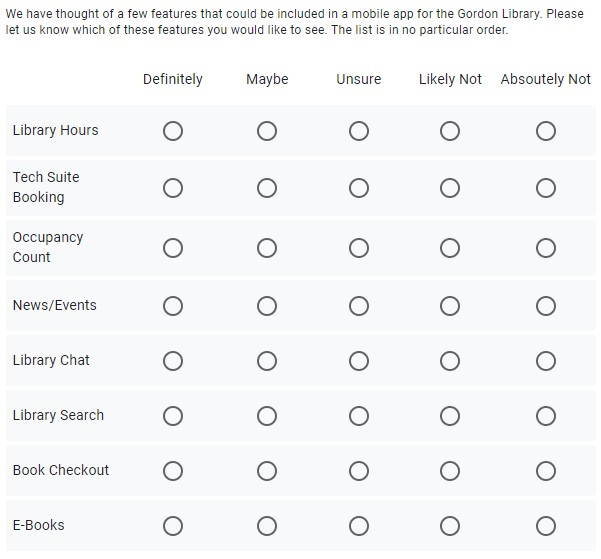
\includegraphics[width = \textwidth, height = \textheight, keepaspectratio]{assets/img/Initial Survey Q7.jpg}
\end{figure}
\newline


\noindent\textbf{Question 8: Do you suggest any additional features not shown above?}
\paragraph{}
Your answer
\newline


\noindent\textbf{Question 9: What other apps do you use that give you a pleasant user experience?}
\newline
To provide the highest quality mobile app for our library, please let us know what apps you enjoy using to use as references.
\begin{itemize}
    \item Spotify
    \item YouTube
    \item Outlook
    \item Instagram
    \item Facebook
    \item Snapchat
    \item Tiktok
    \item Uber
    \item Twitch
    \item Twitter
    \item CNN
    \item Fox News
    \item Gmail
    \item Disney+
    \item HBO Max
    \item Amazon
    \item Amazon Video
    \item Minecraft Mobile Edition?
    \item Venmo
    \item Facebook Messenger
    \item Hulu
    \item DoorDash
    \item Coinbase
    \item Walmart
    \item Reddit
    \item Uber Eats
    \item Paypal
    \item CBS
    \item Other:
\end{itemize}
\newline


\noindent\textbf{Question 10: Would you be willing to participate as a volunteer to test our mobile library app over the next two terms? If so, please provide us with your WPI email in the next section.}
\newline
As we progress in the development of this mobile library app, we will be requiring a test group willing to volunteer and test the various stages of our app.
\begin{itemize}
    \item Yes
    \item No
\end{itemize}
\newline


\noindent\textbf{Question 11: Please provide your WPI email (optional) if you would like for us to contact you.}
\newline
This is completely optional and you may choose to remain anonymous for the survey. Otherwise, please use your WPI email.
\newline


\noindent\textbf{Question 12: Do you have any additional comments about the development of this library app?}
\paragraph{}
Your answer